\documentclass{homework}
\usepackage[utf8]{inputenc}

\usepackage{graphicx}
\usepackage{float}
\graphicspath{ {./images/} }

\usepackage{amsmath}
\usepackage{amssymb}

\title{GPGN470A HW 4: Image Manipulation}
\author{Tyler Singleton}

\begin{document}
\maketitle

% --- Question 2 --- %
\textbf{Question 2:} \\

\begin{figure}[H]
    \centering
    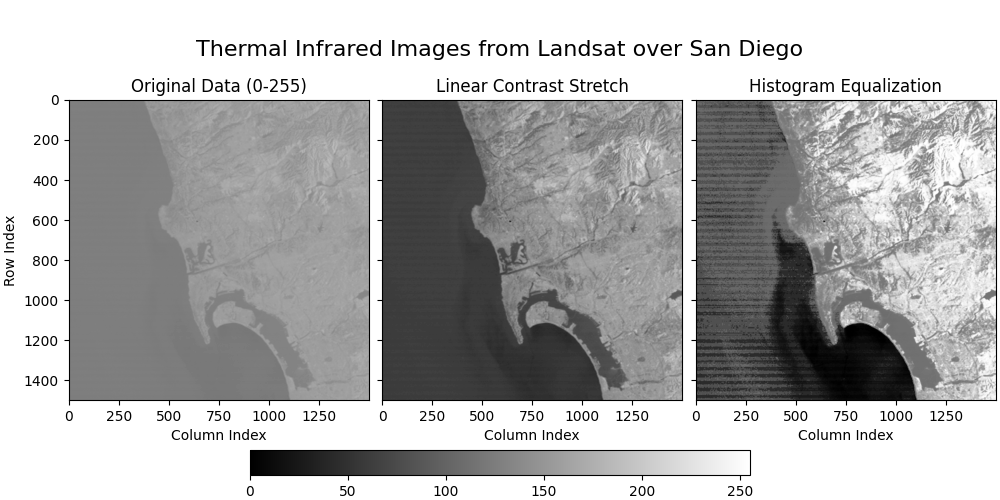
\includegraphics[width=0.85\textwidth]{images/Enhanced_Images.png}
    \caption{Image generated using thermal infrared band from Landsat. The first photo displays no contrast enhancement, middle image utilizes a linear contrast stretch, third image was enhanced using a histogram equalization.}
    \label{fig:Enhanced_Images}
\end{figure}

In this image, the ocean appears to be cooler than the land. This is especially apparent with the waters approaching the San Diego Bay. Additionally, the waters within the San Diego bay are much warmer and closer to the same thermal temperature as surrounding land mass. This may be representative of bay being relatively shallow, and so the waters will warm much quicker. 

\begin{figure}[H]
    \centering
    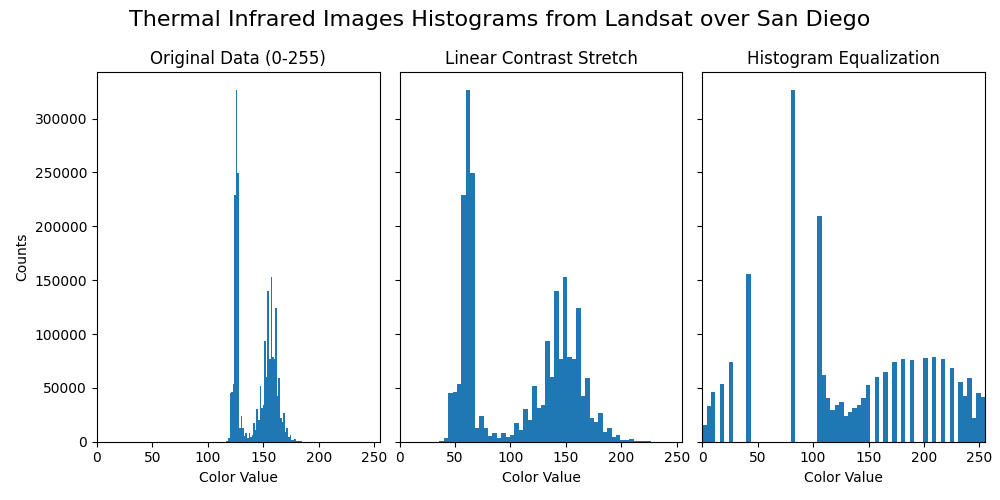
\includegraphics[width=0.85\textwidth]{images/Enhanced_Image_Histograms.png}
    \caption{Histograms from Figure \ref{fig:Enhanced_Images}. The color values are from 0-255 and counts are representative of number of pixels.}
    \label{fig:Enhanced_Histograms}
\end{figure}

Looking at the histograms, the original data has little contrast between features. Most of the color values reside between 120 and 170. A linear contrast provide a greater contrast resolution and allows us to start distinguishing features such as roads, streams, and rivers. The histogram equalization continues to enhance our contrast, but at a cost where noise starts to interfere with interpreting our image. \\

% --- Question 3 ---
\textbf{Question 3:} \\

\begin{figure}[H]
    \centering
    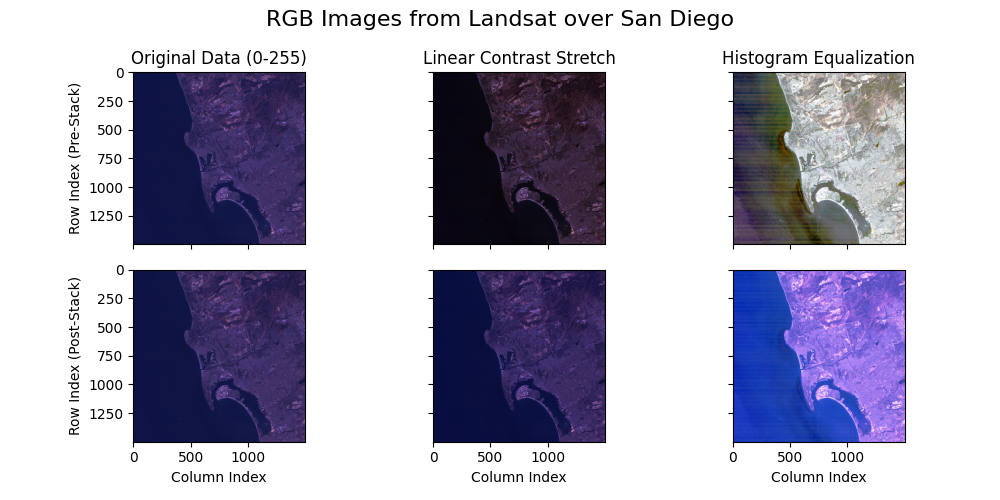
\includegraphics[width=\textwidth]{images/RGB_Enhanced_Images.png}
    \caption{This figure is a composite of band 1, 2, and 3. Enhancements were used pre-stacked (top) and post-stacked (bottom). }
    \label{fig:RGB_Enchanced}
\end{figure}

In Figure \ref{fig:RGB_Enchanced}, the color for our original image looks blue. I believe this to be mainly due to our blue-green band having a larger spread of color values where as green and red are fairly compacted. Processing the image using a linear contrast pre-stack, it begins to more closely resemble reality. The pre-stack histogram equalization greatly distorts from the true color. However, the post-stack histogram equalization does much better and looks the most natural. \\

% --- Question 4 ---
\textbf{Question 4:} \\

 \begin{figure}[H]
     \centering
     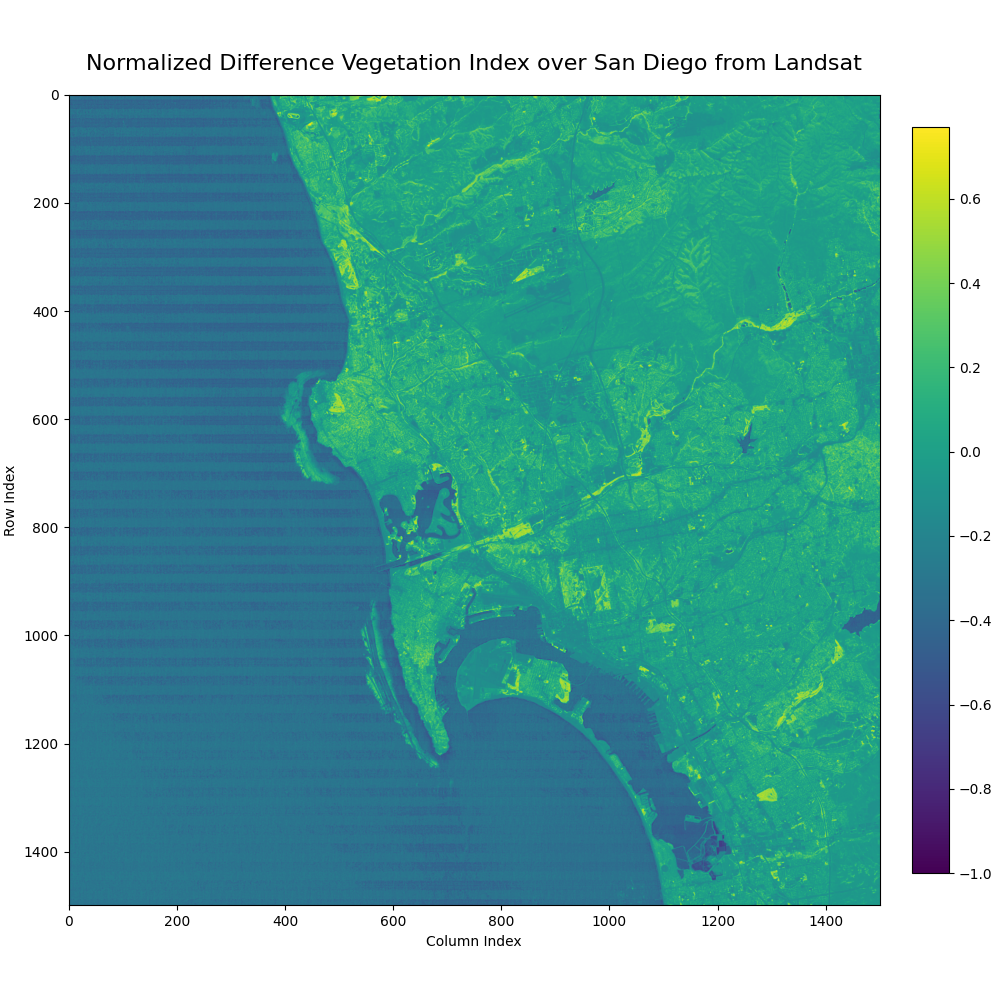
\includegraphics[width=\textwidth]{images/NDVI.png}
     \caption{Normalized difference vegetation index (NDVI) computed using band 3 (red) and 4 (near infrared). }
     \label{fig:NDVI}
 \end{figure}

Compared to our thermal infrared image in question (2), our NDVI provides greater detail of the vegetated areas. For instance, streams and rivers are easier to pick out due to the vegetation growth along their banks; additionally, roads and highways can be distinguished from waters. In the ocean, we can see possibly plant life that was not visible from thermal. But this could also be representative of organic waste and pollution. \\

% --- Question 5 ---
\textbf{Question 5:} \\

\begin{figure}
    \centering
    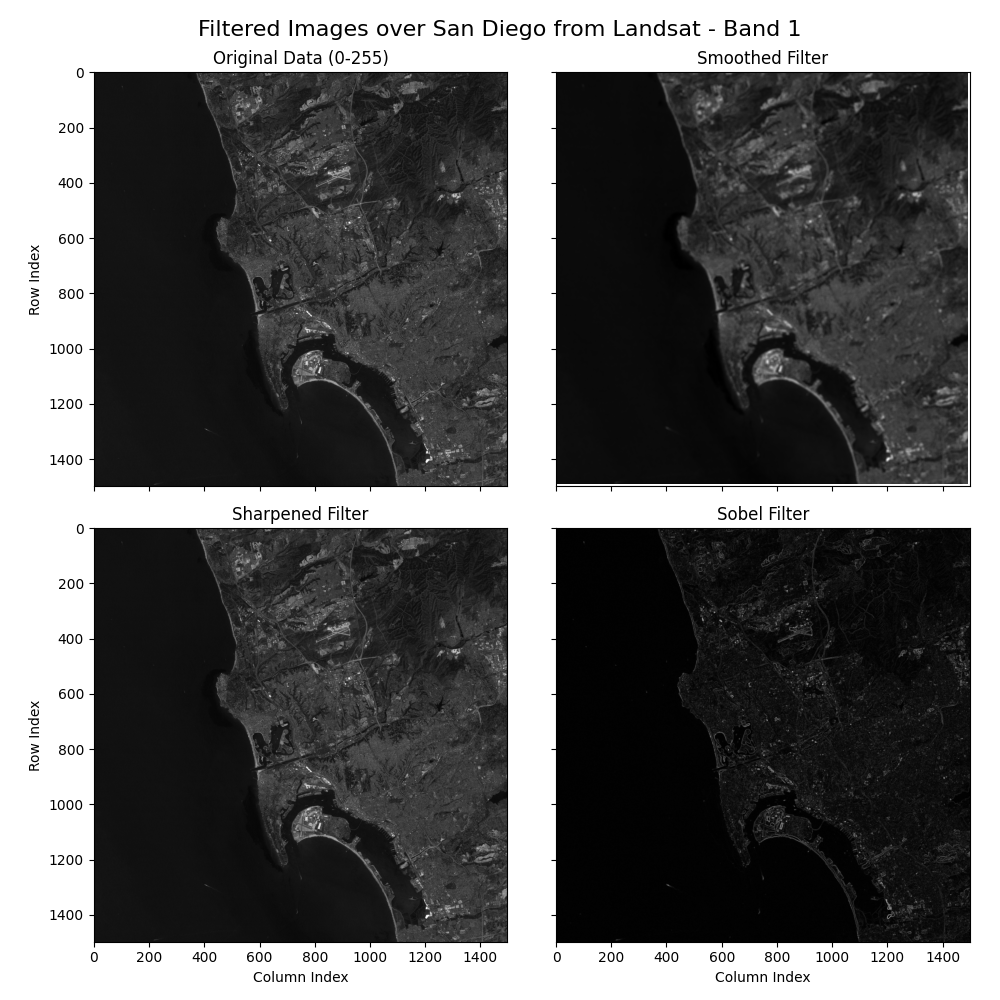
\includegraphics[width=\textwidth]{images/Filtered_Images.png}
    \caption{Using the Blue-Green color band (band 1) from Landsat, these four images highlight different processing filters -- smoothed, sharpened, and sobel.}
    \label{fig:Filtered_Images}
\end{figure}



\end{document}
